\documentclass[11pt]{article}
\usepackage[margin=1in]{geometry}
\usepackage[T1]{fontenc}
\usepackage{lmodern}
\usepackage{amsmath,amssymb,booktabs,graphicx}
\usepackage[round,authoryear]{natbib}
\usepackage[hidelinks]{hyperref}
\usepackage{microtype}
\usepackage{placeins}
\hypersetup{pdfauthor={Nicolas Coquelet},pdftitle={Closing-Line Lab: Registered Football Forecasting}}
\graphicspath{{generated/}{paper/generated/}}
\newcommand{\researchRows}{55476}
\newcommand{\rawFiles}{150}
\newcommand{\valMatches}{11486}
\newcommand{\testMatches}{3754}
\newcommand{\valBets}{4}
\newcommand{\testBets}{2}
\newcommand{\testLoss}{1.007961}
\newcommand{\closingLoss}{1.006958}
\newcommand{\testGap}{0.001003}
\newcommand{\testClv}{-0.026073}
\newcommand{\testProfit}{-0.832686}
\newcommand{\valClv}{-0.039889}
\newcommand{\forwardForecasts}{0}
\newcommand{\forwardBets}{0}
\newcommand{\settledForwardBets}{0}
\newcommand{\scheduledRuns}{2}
\newcommand{\localRuns}{1}
\newcommand{\testNonzeroDays}{2}
\newcommand{\testCalendarDays}{306}
\newcommand{\powerTen}{23821}
\newcommand{\replayError}{1.11e-16}
\newcommand{\testsPassed}{67}
\newcommand{\sourceCommit}{a66736cf5fd4f49e3699cc0b10a9dd0dc5c4f22b}
\newcommand{\registrationCommit}{8b59f2a755a99fc3bc8399c3ef944002a0681cb8}
\newcommand{\originalCommit}{7c16ca0b79f71a30f7820e26289d651d22ecbb58}
\newcommand{\effectThreshold}{0.05}
\newcommand{\creditCap}{400}
\newcommand{\creditReserve}{100}
\newcommand{\oldNullRate}{0.25}
\newcommand{\candidateOneUpper}{0.133057}
\newcommand{\candidateTwoUpper}{0.052782}

\title{Closing-Line Lab: A Registered Football Forecasting Pipeline\\with Negative Historical Results and Sparse Betting Evidence}
\author{Nicolas Coquelet\\CentraleSup\'elec \& ESSEC Business School}
\date{30 October 2026}
\begin{document}
\maketitle
\begin{abstract}
A market-anchored logistic blend achieves outcome log loss \testLoss{} against
\closingLoss{} for de-vigged closing prices on \testMatches{} held-out football matches.
The selected rule places only \testBets{} historical paper bets: mean log closing-line
value (CLV) is \testClv{} and profit is \testProfit{} fictional units. Neither forecast
accuracy nor these sparse bets establish an edge. We compare Dixon--Coles, Elo and market
features using chronological fits over a privately cached dataset of \researchRows{}
rows. Selection is registered before the final-season evaluation, with two prospectively
excluded schema-previewed fixtures. Sparse date-bootstrap quantiles do not support significance testing; two synthetic-only
inference candidates fail their calibration screen. The pilot therefore reports descriptive
CLV without a confirmatory rejection rule. A prospective
pipeline records forecasts and near-kickoff quotes using hash chains and GitHub server
receipts, with durable API-credit reservations. At the reporting snapshot there are
\forwardForecasts{} forward forecasts and \settledForwardBets{} settled forward bets.
The historical comparison is negative; prospective performance remains unobserved.
\end{abstract}

\section{Introduction}
Football markets provide repeated three-outcome forecasts and an observable later price
against which an earlier quote can be compared. This makes them useful for studying
forecasting discipline, abstention and research provenance. A larger match count does not
ensure independent observations, enough selected bets, or reliable inference. A strategy
that largely reproduces market probabilities may forecast many matches while almost never
crossing a meaningful value threshold.

Our question is whether a fixed model can obtain positive mean log CLV on decisions
recorded before kickoff. The closing quote is a benchmark, rather than a known fair
probability or proof of profitability. Our experiment is paper only. It creates no
bookmaker account, order or transfer of money.

The contributions are: (i) a chronological comparison of a time-decayed Dixon--Coles
model, Elo, and a market-anchored logistic blend, including every declared validation
candidate and the negative held-out result; (ii) an auditable prospective protocol that
binds quotes to pre-kickoff server receipts and reserves data credits remotely before
transmission; and (iii) synthetic calibration checks that show why the sparse betting sample
cannot support the proposed CLV significance tests.

\section{Related work}
\citet{dixon1997} model football scores with dynamic team strengths and a correction for
low-score dependence. We implement that structure with explicit regularization and a
fixed fitting cadence; we do not claim to reproduce their empirical betting returns.
\citet{kaunitz2017} study strategies based on bookmakers' own prices and practical betting
restrictions. Their work motivates a market-based comparison, but does not establish an
edge for this dataset, selection rule or later market regime.

Bootstrap resampling originates in \citet{efron1979}. Resampling match dates preserves
within-date groups, but percentile endpoints from very few dates do not automatically
have their nominal coverage. We demonstrate the failure for the original two-date rule
and retain its endpoints as descriptive quantities. \citet{bailey2014} develop a Deflated
Sharpe Ratio (DSR) correction for selection and non-normal returns. Our trial accounting and variance floor are additional conventions. We withhold DSR
inference from the sparse test sample.

\section{Data}
\subsection{Historical source and access}
The local dataset contains \researchRows{} unique rows from \rawFiles{} season--league
CSV downloads from \href{https://football-data.co.uk/}{football-data.co.uk}. It covers the
top two divisions in England, Germany, Italy, Spain and France, from 2012/13 through the
cached partial 2026/27 season. Not all rows have all odds fields or enter evaluation.
We credit the provider and retain download URLs, byte counts and SHA-256 digests in a
committed manifest. Downloads were sequential and cached once for the owner's private,
non-commercial research under the documented owner decision. That decision is not an
additional licence from the provider.

Raw CSVs, processed rows, historical predictions and individual historical bets remain
local and ignored. Public artifacts consist of code, aggregate metrics/figures, manifests
and fitted parameters. The notices distinguish this research use from unrestricted
commercial or automated redistribution. Reproduction of exact historical rows requires
the matching private cache; a mutable source URL cannot guarantee recovery of a lost snapshot.

\subsection{Prices and timing assumptions}
Historical decision prices are B365 non-closing fields; the primary later benchmark is
AvgC. Non-closing fields are periodically captured snapshots, not verified opening odds.
The CSVs do not supply auditable publication times for those prices. We therefore use a
24-hour-before-kickoff decision proxy and make only a conditional as-of claim about result
features. Results with known kickoff times become available after 12 hours; date-only
records after 36 hours. These assumptions do not reconstruct executable historical prices.
Pinnacle historical fields are excluded because of the provider's feed-staleness warning.

Outcome scores use identical complete closing-price and known-result masks for model
and benchmark. The selected test predictions contain zero missing closing triples and one missing result.
The frozen rule abstains on that unresolved match; any selected unresolved stake remains
pending exposure rather than a realized loss.

\subsection{Prospective source}
The Odds API v4 supplies official programmatic event discovery, EU head-to-head quotes and
scores \citep{oddsdocs}. The forward population is EPL and Championship, chosen for
coverage and budget before examining strategy returns. A macOS LaunchAgent runs hourly at minute 05, with GitHub Actions at minute 17 UTC as
fallback. Both use the same collection and publication entry point. It attempts the first complete fresh decision quote 23--25 hours
before kickoff and later a snapshot 15--75 minutes before kickoff. Quotes older than
30 minutes are rejected. Decisions prefer Pinnacle then Betfair Exchange EU; closes prefer
Betfair Exchange EU then Pinnacle. No best-price search is performed.

Here ``closing line'' means the last captured pre-kickoff snapshot with a valid server
receipt, not the literal last exchange price. Each observation records bookmaker, update
and retrieval times, source hash and actual snapshot-to-kickoff gap. Delayed scheduling,
missing coverage and budget restrictions can leave observations absent. Missing observations
are never backfilled using post-match information.

\section{Method}
\subsection{Forecasts}
For decimal odds $o_j$, proportional de-vigging gives
\begin{equation}
q_j=\frac{o_j^{-1}}{\sum_{k\in\{H,D,A\}}o_k^{-1}}.
\end{equation}
The market-only forecast uses these probabilities. Dixon--Coles estimates home and away
goal rates from centered attack/defence effects, a common level and home advantage.
Its weighted Poisson likelihood applies the four low-score adjustments of
\citet{dixon1997}. We use a 365-day half-life, a 1,095-day window, monthly refits, ridge
penalty 0.02 and $\rho\in[-0.1,0]$. Rates are clipped to $[e^{-2},e^2]$ and outcome
probabilities normalize a 0--30 goal grid. Fits require at least 100 earlier league matches;
optimizer failure stops evaluation.

Elo starts at 1,500 per team/league, uses $K=20$, home advantage 75, and Davidson-style
three-way probabilities proportional to $(r,0.7\sqrt r,1)$, where
$r=10^{(R_H+75-R_A)/400}$. Updates use only results available before the decision.
The blend uses shared residual weights and outcome intercepts around the market anchor:
\begin{equation}
p_j\propto \exp\!\left[\log q_j+b_j+
 w_{DC}(\log p_{DC,j}-\log q_j)+w_E(\log p_{E,j}-\log q_j)\right].
\end{equation}
The two shared weights and three intercepts have bounds $[-1,1]$ and ridge penalty 10.
A July fit uses completed earlier seasons only, with at least 1,000 feature rows.
There is no current-season coefficient optimization.

Historical DC/Elo features update under the fixed chronological rules. Forward parameters
are exported once after the original registration and test evaluation: DC/Elo use results
available at export, while blend fitting labels end before the test season. All parameters
then stay fixed. This deliberately introduces cadence and price-source shifts; hosted jobs
never download football-data rows or retrain the model.

\subsection{Paper selection, account and metrics}
Choose at most one side maximizing $p_j\tilde o_j-1$, ties in H/D/A order, with odds in
$[1.2,10]$ and edge at least \effectThreshold. Exchange effective odds are
$\tilde o=1+0.98(o-1)$; book odds are unchanged. The account begins at 100 fictional units.
Stake fraction is $\min(0.01,0.25(p_j\tilde o_j-1)/(\tilde o_j-1))$, subject to available
cash and a 10\% open-exposure cap. Open stakes are valued at cost; future winnings cannot
fund simultaneous decisions. Unknown outcomes remain pending and are excluded from
realized profit, ROI and the settled-bet CLV summary without removing them before selection.

Primary log CLV is $\log(o_{\mathrm{taken}}/o_{\mathrm{close}})$ on the selected side,
unweighted across settled bets with an observed close. Secondary checks use
$\log(o_{\mathrm{taken}}q_{\mathrm{close}})$ and same-book raw CLV where available. Raw
cross-book CLV can reflect margin differences. Outcome log loss and summed multiclass
Brier score compare forecasts with de-vigged closing probabilities on the same matches.
Closing-distribution cross entropy is a separate market-distance diagnostic. Neither
paper P\&L nor displayed quotes establish executable fills, depth or attainable returns.

\section{Protocol}
\subsection{Splits, registration and trial accounting}
Features begin in 2015/16 after initial history. Validation spans 2022/23--2024/25; the final
full season 2025/26 is evaluated after the original \texttt{forward-v1} tag. Four forecast
families crossed with minimum edges 0.03/0.05 form eight declared candidates. Selection
minimizes validation outcome log loss, with exact ties choosing the higher threshold.
Thresholds do not change forecast probabilities; ties therefore do not select on CLV or
profit. All candidates are retained. No league, side or lead-time search is used.

Two test fixtures had been displayed for schema inspection before fitting and were
prospectively excluded from primary test metrics. Thus the full season was not fully
blinded. Earlier test results may enter later test features under the fixed as-of rule;
aggregate test metrics cannot guide model or threshold changes. The blend and parameter file remain fixed.

All candidates and iterations, including failures, enter the trial registry. Historical
DSR diagnostics retain evaluation-time counts; forward reports use the growing registry.
This conservative bookkeeping does not estimate independent searches or control familywise
error. No confirmatory model-comparison test or superiority claim is made.

The active \texttt{forward-v1.3} protocol withdraws confirmatory CLV inference before any
forward forecast. Original tags and result artifacts remain archived.

\subsection{Sparse inference and calibration}
A positive lower 95\% date-bootstrap percentile endpoint is not a valid positive-CLV
test in this sparse setting. With two independent symmetric continuous zero-mean observations,
the resampled support lies between those two observations. The lower percentile is positive
when both are positive, which occurs with probability \oldNullRate. Coverage of zero is
only one half. Nominal percentile labels therefore gave misleading inference.

We retain the resampling endpoints as descriptive quantiles. Two replacement candidates
were screened using synthetic data only: bet-weighted weekly means, Bartlett HAC variance
with four lags, a Student-$t$ critical value, unequal week sizes, and increasing minimum
information. The null grid combines normal, Student-$t(5)$ and negative centered lognormal
innovations, weekly AR(1) coefficients 0, 0.3 and 0.6, and 30, 60 or 120 populated weeks.
Each scenario uses 10,000 replications with seed 20261029 and a burn-in. Acceptance requires
every scenario's Wilson 95\% upper false-positive bound to be at most 0.05. This empirical
screen would not establish universal validity even if passed.

Both candidates fail (Table~\ref{tab:nulls}). This pilot therefore reports no inferential
CLV interval or positive-evidence decision, regardless of sample size. A future confirmatory
study needs a validated preregistration. DSR is withheld below 30 nonzero return days or
60 calendar days; its original sparse-sample arithmetic remains archived.

\subsection{Forward inclusion and publication}
The planned decision window is 29 October 2026 through 29 January 2027 exclusive (UTC).
Inclusion is by decision time: existing forecasts can receive closes and settlement after
the window ends. There is no performance-based stopping or extension.

Forecasts and closing snapshots append to a SHA-256 chain. Publication checks a kickoff
buffer, pushes without rewriting history, and dispatches an audit. A GitHub run's server
creation time and head SHA must bind the exact ledger content before kickoff; local git
author timestamps are insufficient. Settlement must reference the latest receipted close
and replay its prices, bookmaker, gap and raw/secondary CLV. Without such evidence every
close-derived field is null, although a known outcome may settle P\&L.

A shared remote branch serializes runners with a compare-and-swap lease and records
completed UTC hours, preventing duplicate work across Mac and GitHub executions. The same
branch records a credit reservation before each paid HTTP call. A killed runner leaves its
lease locked for manual reconciliation; leases never expire automatically. Ambiguous failure leaves a pending reservation and blocks paid requests even
on a new runner or after a provider reset. Manual reconciliation retains ambiguous charges;
paid calls are not retried. The \creditCap{}-credit calendar-month cap and
\creditReserve{}-credit provider reserve leave headroom on the intended free plan. Free
fixture discovery and due-window gating reduce requests. Actual coverage is not guaranteed.

\section{Results}
\subsection{Historical forecast and selection results}
Table~\ref{tab:validation} includes every declared validation strategy. The selected blend
is nearer to closing log loss than DC or Elo, but remains worse than the closing baseline.
The higher threshold yields only \valBets{} validation bets. This selection rule is fixed
before inspecting the final-season aggregate and is retained despite weak betting power.
\begin{table}[htbp]
\centering\small
\begin{tabular}{lrrrr}
\toprule
Model & Edge & Log loss & Bets & Mean log CLV \\
\midrule
Market & 0.03 & 1.006368 & 0 & --- \\
Market & 0.05 & 1.006368 & 0 & --- \\
Dixon--Coles & 0.03 & 1.025917 & 3401 & -0.004311 \\
Dixon--Coles & 0.05 & 1.025917 & 3192 & -0.004204 \\
Elo & 0.03 & 1.025936 & 3465 & -0.007975 \\
Elo & 0.05 & 1.025936 & 3272 & -0.007094 \\
Blend & 0.03 & 1.005764 & 14 & -0.048238 \\
Blend & 0.05 & 1.005764 & 4 & -0.039889 \\
\bottomrule
\end{tabular}

\caption{All declared validation candidates on the common \valMatches{} scored matches.
An undefined CLV mean is shown as a dash. No threshold is chosen on CLV.}
\label{tab:validation}
\end{table}

Table~\ref{tab:scores} shows paired forecast scores. On \testMatches{} test matches, the
blend's log-loss gap to closing is \testGap{} nats, a deterioration. Brier scores also
favor closing at their point estimates. Calibration bins in Figure~\ref{fig:calibration}
are descriptive and do not establish betting value.
\begin{table}[htbp]
\centering\small
\begin{tabular}{lrrr}
\toprule
Population / forecast & Matches & Log loss & Brier \\
\midrule
Validation: blend & 11486 & 1.005764 & 0.601869 \\
Validation: close & 11486 & 1.002834 & 0.599915 \\
Test: blend & 3754 & 1.007961 & 0.603416 \\
Test: close & 3754 & 1.006958 & 0.602787 \\
\bottomrule
\end{tabular}

\caption{Selected blend and proportional de-vigged closing benchmark on identical masks.
Lower log loss and summed multiclass Brier are better.}
\label{tab:scores}
\end{table}
\begin{figure}[htbp]
\centering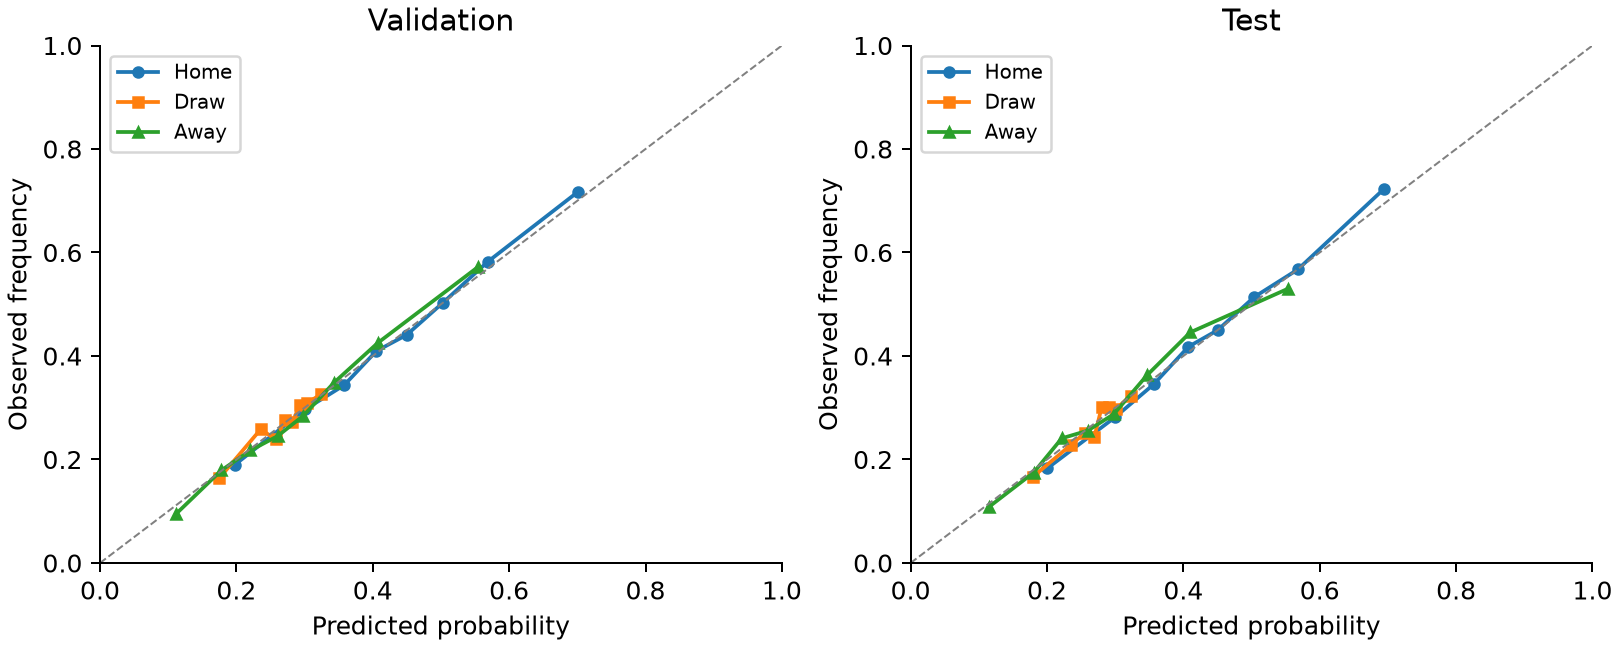
\includegraphics[width=\linewidth]{calibration.png}
\caption{H/D/A calibration from committed aggregate quantile bins. Curves show mean
predicted probability against observed frequency, without inferential error bars.}
\label{fig:calibration}
\end{figure}

\FloatBarrier
\subsection{Selected bets, replay and power}
The \testBets{} selected test bets both lose. Their mean log CLV is \testClv{} and paper
profit is \testProfit{} units (Table~\ref{tab:bets}). ROI is on staked capital, not the
entire initial account. The two-date bootstrap endpoints are the individual CLV extremes;
they are not calibrated confidence limits. DSR is not estimable with \testNonzeroDays{}
nonzero return days despite \testCalendarDays{} calendar observations.
\begin{table}[htbp]
\centering\small
\begin{tabular}{lrr}
\toprule
Selected-rule quantity & Validation & Test \\
\midrule
Settled bets & 4 & 2 \\
Pending bets & 0 & 0 \\
Mean log CLV & -0.039889 & -0.026073 \\
Bootstrap 2.5\% quantile & -0.086783 & -0.159849 \\
Bootstrap 97.5\% quantile & 0.016521 & 0.107702 \\
Paper profit (units) & 2.306993 & -0.832686 \\
ROI on settled stakes & 0.970305 & -1.000000 \\
Nonzero return days & 4 & 2 \\
DSR inference & Not estimable & Not estimable \\
\bottomrule
\end{tabular}

\caption{Selected-rule betting summaries. Bootstrap endpoints are descriptive quantiles
from date resampling, not reliable confidence limits. Fictional units have no cash value.}
\label{tab:bets}
\end{table}

An isolated full-feature replay reproduces all declared validation and selected test
estimates, with maximum prediction deviation \replayError.

A normal-approximation planning calculation based on only \valBets{} validation bets
suggests \powerTen{} bets for 10 log-CLV basis points at one-sided 5\% size and 80\% power.
This is an unstable variance extrapolation, not a reliable sample-size requirement or a
validated test design. Two test bets cannot estimate planning power. The proposed
three-month window is unlikely to identify a small edge for such a sparse rule.

\subsection{Null checks and prospective status}
Both inference candidates fail (Table~\ref{tab:nulls}, Figure~\ref{fig:nulls}). The larger
critical parameter reduces rejection, but its worst upper bound, \candidateTwoUpper{}, still
exceeds the screen. Neither nominal setting is a validated confidence level.
\begin{table}[htbp]
\centering\scriptsize
\begin{tabular}{lrrrrl}
\toprule
Candidate & Min. weeks & Critical parameter & Max. FPR & Upper bound & Screen \\
\midrule
1 & 30 & 0.990 & 0.126400 & 0.133057 & FAIL \\
2 & 60 & 0.999 & 0.048400 & 0.052782 & FAIL \\
\bottomrule
\end{tabular}

\caption{Synthetic-only inference screen. FPR is rejection under the zero-mean null.
``Critical parameter'' specifies the candidate's nominal interval calculation, not achieved
coverage. Both candidates also require 100 bets. The upper bound is Wilson 95\% per scenario.}
\label{tab:nulls}
\end{table}
\begin{figure}[htbp]
\centering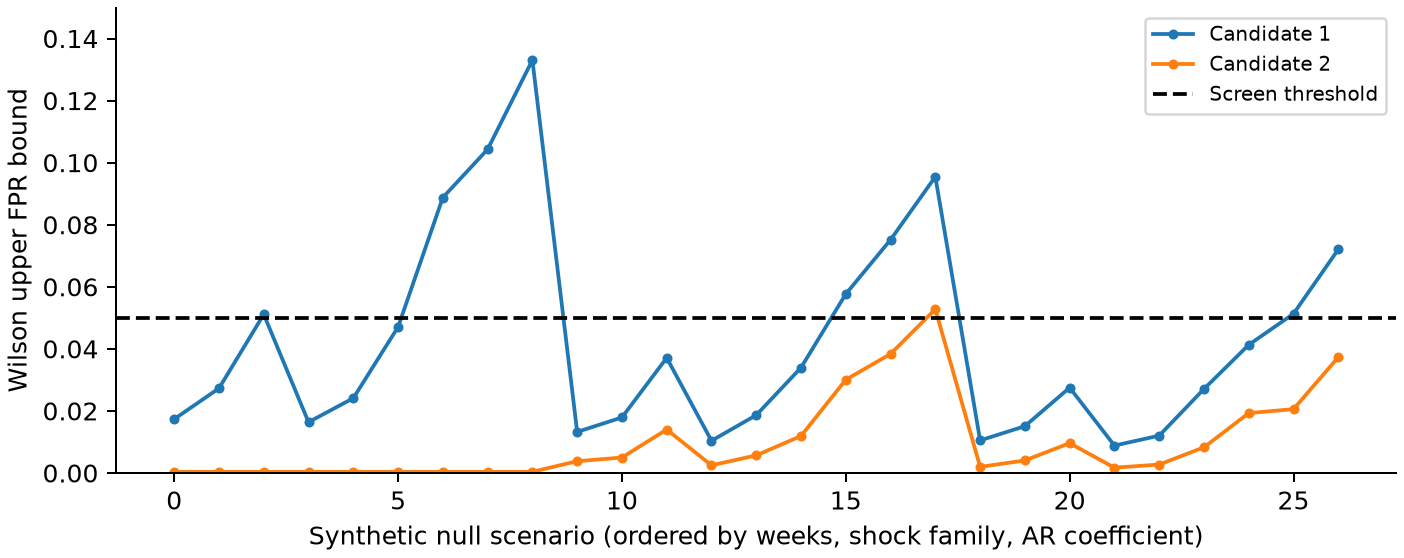
\includegraphics[width=0.92\linewidth]{null_screen.png}
\caption{Upper false-positive bounds across the complete synthetic scenario grid.
Ineligible sample sizes never reject. Every scenario must satisfy the dashed threshold.}
\label{fig:nulls}
\end{figure}

At the committed reporting snapshot there are \forwardForecasts{} forward forecasts,
\forwardBets{} selected paper bets and \settledForwardBets{} settled forward bets.
The live GitHub query records \scheduledRuns{} successful scheduled executions; the Mac
installation has \localRuns{} verified real cycle. These operational checks do not establish
an on-time forecast, close or settlement. Hosted jobs are currently blocked by a GitHub
account billing restriction; the Mac runner remains installed. Backtest versus forward
performance is not yet comparable.
\FloatBarrier

\section{Limitations}
Historical prices lack trustworthy as-of publication times. Result-availability proxies,
cross-book margins and a closing market that need not be efficient constrain interpretation.
The test season contains declared schema-preview exceptions. Data reuse across chronological
features is intentional, but does not create independent match observations. Abstention
leaves the selected strategy with too few bets for confirmatory inference.

Forward parameters remain fixed while historical DC/Elo updated; source and cadence shifts
may dominate a future comparison. Hosted schedules can be delayed or dropped; the Mac runner also depends on wakefulness,
network access and an available shell credential. Either runner can be blocked by an
unreconciled remote lease or reservation. The observed
close can precede the literal final line substantially; source update gaps are reported
separately. API quotas, quote completeness, name mappings and outages affect inclusion.
The scores endpoint's limited lookback can leave outages unresolved. Missingness may be
systematic, so complete-case CLV need not describe all planned decisions.

Indicative quotes, a fixed exchange commission and fictional stakes do not model depth,
limits, slippage or account restrictions. Neither CLV nor paper returns establish attainable
profit. Hash chains and server receipts are tamper-evident against retained history, not
immutable: repository owners can delete history and runs. Private evidence requires access.
The public aggregate artifacts do not permit exact row-level replay without the private
source cache. Synthetic null scenarios are finite and cannot prove coverage under arbitrary
heavy tails or dependence; disabling confirmation is the supported decision here.

\section{Reproducibility}
The original pre-test registration is commit
\texttt{\originalCommit}; active prospective protocol v1.3 is
\texttt{\registrationCommit}. Tables, numerical macros and figures are generated by
\texttt{paper/make\_tables.py} from Git-committed aggregate artifacts at
\texttt{\sourceCommit}. Their SHA-256 digests and the generator hash are saved in
\texttt{paper/generated/provenance.json}. Displayed decimals use a consistent rounding-to-nearest
rule; machine-readable artifacts retain full precision.

Python 3.12 dependencies are locked with uv. Tests cover as-of features, de-vigging, CLV,
ledger evidence, budget loss across fresh runners, pending stakes and end-window closing.
The recorded engineering snapshot passes \testsPassed{} tests. Commands from the repository
root are:
\begin{verbatim}
uv sync --frozen
make check test
OPENBLAS_NUM_THREADS=1 OMP_NUM_THREADS=1 uv run cll replay \
  --output-dir runs/reviewer-replay --rebuild-features
uv run python scripts/calibrate_inference.py --min-weeks 30 \
  --critical-coverage 0.99 --output runs/candidate1.json
uv run python scripts/calibrate_inference.py --output runs/candidate2.json
make verify
uv run python paper/make_tables.py
tectonic -X compile paper/main.tex
\end{verbatim}
The replay command needs the authorized local cache and writes isolated ignored outputs;
it does not rerun selection or overwrite registered artifacts. Null simulations need no
market data. The paper generator reads committed blobs directly, never uncommitted local
rows. Reference metadata and identifiers were resolved through Crossref, the arXiv API or
official documentation and retained in \texttt{paper/reference\_verification.json}.

\section{Conclusion}
The selected market-anchored blend does not beat the closing benchmark at held-out point
estimates. Its sparse selected bets show negative CLV and losses but cannot support precise
inference. Two synthetic inference candidates fail their calibration screen; the pilot remains
descriptive. The prospective infrastructure
and retained provenance support a future evaluation, but no operating forward edge has yet
been demonstrated.

\bibliographystyle{plainnat}
\bibliography{refs}
\end{document}
